\documentclass[conference]{worldcomp}

\usepackage[hmargin=.75in,vmargin=1in]{geometry}
\usepackage[american]{babel}
\usepackage[T1]{fontenc}
\usepackage{times}
\usepackage{caption}

%%% Below packages are recommended to use for better results and compatible with the worldcomp.cls
\usepackage{textcomp}
\usepackage{epsfig,graphicx}
%\usepackage{graphicx}
\usepackage{xcolor}
\usepackage{amsfonts,amsmath,amssymb}
\usepackage{fixltx2e} % Fixing numbering problem when using figure/table* 
\usepackage{booktabs}
\usepackage{colortbl}
\pagestyle{plain}

\newcommand{\pathname}     {common/}
\newcommand{\fullpath}     {\pathname}

% http://stackoverflow.com/questions/3208691/how-to-identify-equation-and-subsection-counters-in-latex
% \newtheorem{myDefinition}[section]{Definition}
\newtheorem{myDefinition}{Definition}
\newtheorem{myTheorem}{Theorem}
\newtheorem{myLemma}{Lemma}

\numberwithin{equation}{section}
\numberwithin{myTheorem}{section}

% other definitions
%% shades of gray
\definecolor{darkgray}{gray}{0.25}
\definecolor{medgray} {gray}{0.75}
\definecolor{ltgray}  {gray}{0.90}
\definecolor{vltgray} {gray}{0.95}

%\definecolor{rangecolor} {blue}
%\definecolor{nullcolor}  {red}

%% basic color directives
\newcommand{ \bl }[1]        {{\color{blue}   {#1}}}
\newcommand{ \bk }[1]        {{\color{black}  {#1}}}
\newcommand{ \rd }[1]        {{\color{red}    {#1}}}
\newcommand{ \gr }[1]        {{\color{green}  {#1}}}
\newcommand{ \pr }[1]        {{\color{purple} {#1}}}
\newcommand{ \mg }[1]        {{\color{medgray}{#1}}}

%% numbers blue
\newcommand{ \bzero }[0]     { \bl{ 0 } }
\newcommand{ \bone }[0]      { \bl{ 1 } }
\newcommand{ \btwo }[0]      { \bl{ 2 } }
\newcommand{ \bthree }[0]    { \bl{ 3 } }
\newcommand{ \bfour }[0]     { \bl{ 4 } }
\newcommand{ \bfive }[0]     { \bl{ 5 } }
\newcommand{ \bsix }[0]      { \bl{ 6 } }
\newcommand{ \bseven }[0]    { \bl{ 7 } }
\newcommand{ \beight }[0]    { \bl{ 8 } }
\newcommand{ \bnine }[0]     { \bl{ 9 } }
\newcommand{ \bminus }[0]    { \bl{ - } }
\newcommand{ \bstar }[0]     { \bl{ * } }
\newcommand{ \bi }[0]        { \bl{ i } }
\newcommand{ \bmone }[0]     { \bl{-1 } }
\newcommand{ \bmi }[0]       { \bl{-i } }
\newcommand{ \bmo }[0]       { \bl{-1 } }

\newcommand{ \bdots }[0]     { \bl{ \dots } }


%% numbers red
\newcommand{ \rzero }[0]     { \rd{ 0 } }
\newcommand{ \rone }[0]      { \rd{ 1 } }
\newcommand{ \rtwo }[0]      { \rd{ 2 } }
\newcommand{ \rthree }[0]    { \rd{ 3 } }
\newcommand{ \rfour }[0]     { \rd{ 4 } }
\newcommand{ \rfive }[0]     { \rd{ 5 } }
\newcommand{ \rsix }[0]      { \rd{ 6 } }
\newcommand{ \rseven }[0]    { \rd{ 7 } }
\newcommand{ \reight }[0]    { \rd{ 8 } }
\newcommand{ \rnine }[0]     { \rd{ 9 } }
\newcommand{ \rminus }[0]    { \rd{ - } }
\newcommand{ \rstar }[0]     { \rd{ * } }
\newcommand{ \rmone }[0]     { \rd{-1 } }

\newcommand{ \rdots }[0]     { \rd{ \dots } }

%% numbers medium gray
\newcommand{ \gzero }[0]     { \mg{ 0 } }
\newcommand{ \gone }[0]      { \mg{ 1 } }
\newcommand{ \gtwo }[0]      { \mg{ 2 } }
\newcommand{ \gthree }[0]    { \mg{ 3 } }
\newcommand{ \gfour }[0]     { \mg{ 4 } }
\newcommand{ \gfive }[0]     { \mg{ 5 } }
\newcommand{ \gsix }[0]      { \mg{ 6 } }
\newcommand{ \gseven }[0]    { \mg{ 7 } }
\newcommand{ \geight }[0]    { \mg{ 8 } }
\newcommand{ \gnine }[0]     { \mg{ 9 } }
\newcommand{ \gminus }[0]    { \mg{ - } }
\newcommand{ \goplus }[0]    { \mg{ \oplus } }

%% numbers black
\newcommand{ \bs }[0]        { {\bk{*}} }
\newcommand{ \bkzero }[0]    { {\bk{0}} }

% nums
\newcommand{ \bnum }[0]      { \bl{ \num } }
\newcommand{ \rnum }[0]      { \rd{ \num } }
\newcommand{ \gnum }[0]      { \mg{ \num } }

\endinput  %  -  -  -  -  -  -  -  -  -  -  -  -  -  -  -  -  -  -  -  -
\newcommand{\paren}[1]   { \left(  #1 \right) }
\newcommand{\inner}[2]   { \langle #1 \overline{#2} \rangle }
\newcommand{\innerx}[2]  { \langle #1 | #2 \rangle }
\newcommand{\brac}[1]    { \left[  #1 \right] }
\newcommand{\lst}[1]     { \left\{ #1 \right\} }

\endinput  %  -  -  - -  -  - -  -  - -  -  - -  -  - -  -  - -  -  - -  -  -
\input{\fullpath/"matrix basics"}
\newcommand{\abs}[1]     {\left| #1 \right|}
\newcommand{\norm}[1]    {\left\lVert #1 \right\rVert}
\newcommand{\normo}[1]   {\left\lVert #1 \right\rVert_{1}}
\newcommand{\normt}[1]   {\left\lVert #1 \right\rVert_{2}}
\newcommand{\normi}[1]   {\left\lVert #1 \right\rVert_\infty}
\newcommand{\normp}[1]   {\left\lVert #1 \right\rVert_{p}}
\newcommand{\normf}[1]   {\left\lVert #1 \right\rVert_F}
\newcommand{\normtL}[1]  {\left\lVert #1 \right\rVert_{L^{2}}}
\newcommand{\normtl}[1]  {\left\lVert #1 \right\rVert_{l^{2}}}

\newcommand{\norms}[1]   {\left\lVert #1 \right\rVert^{2}}
\newcommand{\normos}[1]  {\left\lVert #1 \right\rVert_{1}^{2}}
\newcommand{\normts}[1]  {\left\lVert #1 \right\rVert_{2}^{2}}
\newcommand{\normis}[1]  {\left\lVert #1 \right\rVert_\infty^{2}}
\newcommand{\normps}[1]  {\left\lVert #1 \right\rVert_{p}^{2}}
\newcommand{\normfs}[1]  {\left\lVert #1 \right\rVert_F^{2}}
\newcommand{\normtLs}[1] {\left\lVert #1 \right\rVert_{L^{2}}^{2}}
\newcommand{\normtls}[1] {\left\lVert #1 \right\rVert_{l^{2}}^{2}}


\endinput %-------------------------------
% bys
\newcommand{\by}[2]      {#1 \times #2}
\newcommand{\byy}[1]     {#1 \times #1}
\newcommand{\bymn}[0]    {\by{m}{n}}
\newcommand{\bymm}[0]    {\byy{m}}
\newcommand{\bynn}[0]    {\byy{n}}
\newcommand{\bynm}[0]    {\by{n}{m}}
\newcommand{\bymr}[0]    {\by{m}{\rho}}
\newcommand{\byrn}[0]    {\by{\rho}{n}}

% vector spaces
\newcommand{\real}[1]    {\mathbb{R}^{#1}}
\newcommand{\cmplx}[1]   {\mathbb{C}^{#1}}
\newcommand{\either}[1]  {\cmplx{#1}}
\newcommand{\ir}[0]      {\in\real{}}
\newcommand{\ic}[0]      {\in\cmplx{}}
\newcommand{\icm}[0]     {\in\cmplxm}
\newcommand{\icn}[0]     {\in\cmplxn}
\newcommand{\icmn}[0]    {\in\cmplxmn}
\newcommand{\irmn}[0]    {\in\realmn}
\newcommand{\icmnr}[0]   {\in\cmplxmnr}
\newcommand{\ints}[0]    {\mathbb{Z}}
\newcommand{\natnum}[0]  {\mathbb{N}}

\newcommand{\iints}[0]   {\in \mathbb{Z}}
\newcommand{\inatnum}[0] {\in \mathbb{N}}

\newcommand{\realall}[3] {\real{\by{#1}{#2}}_{#3} }
\newcommand{\cmplxall}[3]{\cmplx{\by{#1}{#2}}_{#3} }

\newcommand{\realn}[0]   {\real{n}}
\newcommand{\realm}[0]   {\real{m}}
\newcommand{\realmn}[0]  {\real{\bymn}}
\newcommand{\realnn}[0]  {\real{\byy{n}}}
\newcommand{\realmm}[0]  {\real{\byy{m}}}
\newcommand{\realmmr}[0] {\real{\byy{m}}_{\rho}}
\newcommand{\realmmm}[0] {\realmm_{m}}

\newcommand{\cmplxn}[0]  {\cmplx{n}}
\newcommand{\cmplxm}[0]  {\cmplx{m}}
\newcommand{\cmplxnn}[0] {\cmplx{\byy{n}}}
\newcommand{\cmplxmm}[0] {\cmplx{\byy{m}}}
\newcommand{\cmplxmn}[0] {\cmplx{\bymn}}
\newcommand{\cmplxmr}[0] {\cmplx{\bymr}}
\newcommand{\cmplxrn}[0] {\cmplx{\byrn}}
\newcommand{\cmplxmnr}[0]{\cmplx{\bymn}_{\rho}}
\newcommand{\cmplxmmm}[0]{\cmplxmm_{m}}
\newcommand{\cmplxmnm}[0]{\cmplxmn_{m}}
\newcommand{\cmplxnnr}[0]{\cmplxnn_{\rho}}
\newcommand{\cmplxmnn}[0]{\cmplxmn_{n}}

% spans
\newcommand{\spn}[1]     {\text{sp\,} \lst{ #1 }}


\endinput %-------------------------------

% matrices  --   --   --   --   --   --   --   --   --   --   --   --
\newcommand{\A}[1]       { \mathbf{A}^{\rm{#1}} }
\newcommand{\As}[0]      { \mathbf{A}^{\rm{*}} }
\newcommand{\PP}[0]      { \mathbf{P} }
\newcommand{\R}[0]       { \mathbf{R} }
\newcommand{\V}[0]       { \mathbf{V} }
\newcommand{\I}[1]       { \mathbf{I}_{#1} }

\newcommand{\re}[0]      { \text{Re} }
\newcommand{\im}[0]      { \text{Im} }

\newcommand{\half}[0]    { \frac{1} {2} }

% domains  --   --   --   --   --   --   --   --   --   --   --   --
\newcommand{\bigL}[0]    { L^{2} }
\newcommand{\littlel}[0] { l^{2} }

\newcommand{\innerxL}[2] { \langle #1 | #2 \rangle_{\bigL} }
\newcommand{\innerxl}[2] { \langle #1 | #2 \rangle_{\littlel} }

% action over domains
\newcommand{\domL}[0]    { \Omega }
\newcommand{\doml}[0]    { \sigma }

\newcommand{\intcont}[0] { \Omega = \lst{x\in\real{}\colon -1 \le x \le 1} }
\newcommand{\intdisc}[0] { \sigma = \lst{x\colon -1 \le x \le 1} }

\newcommand{\spaceL}[0]  { \bigL (\Omega) }
\newcommand{\spacel}[0]  { \littlel \paren{\sigma} }

\newcommand{\intL}[0]    { \bigL[-1,1]}
\newcommand{\intl}[0]    { \littlel[-1,1] }

% \newcommand{\intdom}[1]  { \int_{\domL} #1(x) \overline{#1}^{*}(x) dx }
% \newcommand{\sumdom}[1]  { \sum_{x\in \doml} #1(x) #1^{*}(x) }
\newcommand{\intdom}[1]  { \int_{\domL}      #1(x) \overline{#1(x)} dx }
\newcommand{\sumdom}[1]  { \sum_{x\in \doml} #1(x) \overline{#1(x)} }

\newcommand{\intdomx}[2] { \int_{\domL} #1(x) \overline{#2(x)} dx }
\newcommand{\sumdomx}[2] { \sum_{x\in \doml}  \overline{#2(x)} \Delta }

% epsilon 
\newcommand{\eps}[0]     {\epsilon}
\newcommand{\egtz}[0]    {\eps > 0}

% stray commands  --   --   --   --   --   --   --   --   --   --   --   --

\newcommand{\sgn}[0]     { \text{sgn } }

% bound angle
\newcommand{\dtwo}[0]    { \overline{\dtwoopen} }
\newcommand{\dtwoopen}[0]{ D_{2} }

% order
\newcommand{\order}[1]   { \mathcal{o}\paren{#1} }
\newcommand{\Order}[1]   { \mathcal{O}\paren{#1} }

\newcommand{\mx}[2]      { \max\limits_{#1 \in \cmplx{ #2 }} }
\newcommand{\mn}[2]      { \min\limits_{#1 \in \cmplx{ #2 }} }

\newcommand{\mxxn}[0]    { \mx{x}{n} }
\newcommand{\mnxn}[0]    { \mn{x}{n} }

\newcommand{\mxball}[0]  { \max\limits_{\normt{x} = 1} }

% is equal?
\newcommand{\iseq}[0]    { \overset{?}{=} }

% map A
\newcommand{\mapa}[1]    { \overset{\A{#1}}{\mapsto} }

% header
\newcommand{\head}[1]    { $\A{}$ & $=$ & $\U{}$ & $\sig{}$ & $\V{*}$ }

% spacings and such
\newcommand{\wfour}[0]   {1.05in}

\endinput %-------------------------------
%\setlength\minrowclearance{4pt} 

%%% Below packages are probably useful for some table-formatting purposes. Compatibility is not yet
%%% tested but probably fine.
%\usepackage{tabularx}
%\usepackage{tabulary}

%%% Using the hyperref package is not really necessary for conference papers, but if your paper includes
%%% a lot of URLs, and you wish them to be line-breakable, it might be useful.  When you need to use the
%%% hyperref package, make sure you set <colorlinks option> = true and all link colors black as shown in
%%% the sample below (the sample calls the ifpdf package, too).
\usepackage{ifpdf} 
\ifpdf
\usepackage[pdftex,naturalnames,breaklinks=true,colorlinks=true,linkcolor=black,citecolor=black,filecolor=black,menucolor=black,urlcolor=black]{hyperref}
\else
\usepackage[dvips,naturalnames,breaklinks=true]{hyperref}
\fi

\columnsep 6mm  %%% DO NOT CHANGE THIS
\newcounter{MYtempeqncnt}


%%   %%   %%   %%   %%   %%   %%   %%   %%   %%   %%   %%   %%   %%   %%   %%   %%   %%   %%   %%
\title{\bf Orthogonality and Computation}           

\author{
{\bfseries D.~M. Topa$^{1,2,3}$ and P.~F. Embid$^{1,2}$}\\
$^1$Department of Mathematics and Statistics, University of New Mexico, Albuquerque, NM, USA\\
$^2$Los Alamos National Laboratory, Los Alamos, NM, USA\\
$^3$Engility Corporation, U.S.A.C.E. Engineer Research and Development Center, \\
Information Technology Laboratory, Vicksburg MS, USA\\
}
%%
%%  copy editing: Courtney Tuminello
%%

%%
%%  technical review: Alan Scheinine, Paul Bennet
%%

\begin{document}

\maketitle 

\begin{abstract}
The property of orthogonality is predicated upon the specifications of a domain and a topology. The orthogonality of the continuum is violated in the computational domain as evidenced by poor convergence and numerical oscillations.
Penalties are significant numerical errors and a substantial increase in computation time. By using linear independence, exact solutions are found in specific instances.
\end{abstract}

\vspace{1em}
\noindent\textbf{Keywords:}
 {\small  orthogonality, linear independence, Hilbert space, Lebesgue integration, domain topology } 

%  +  +  +  +  +  +  +  +  +  +  +  +  +  +  +  +  +  +  +  +  +  +  +  +  +  +  +  +  +  +  +  +  +  +  +
\section{Introduction}
Orthogonality and projection are two facets of the same gem. They are foundation concepts in many areas of science and engineering. For example, the  mathematics of quantum mechanics and quantum field theory are the embodiment of the power of orthogonal projection. The least squares method delivers an orthogonal projection. A great deal of mathematics is based upon orthogonality. Computations are too often corrupted by the inappropriate presumption of orthogonality. This paper explores how this malady distorts numerical computations and presents a more suitable schema.

Common knowledge is that the trigonometric functions $\sin n x$ and $\cos n x$ (and their linear combination $e^{inx}$) are orthogonal over both the continuous domain $\Omega=\lst{x\colon -\pi \le x \le \pi}$ and the uniformly sampled discrete domain $\sigma=\lst{x\colon x_{\nu} = -\pi + \frac{\nu}{n}\pi}_{\nu=0}^{2n}$. A branch of mathematics built on these principles is  Fourier analysis, which approximates arbitrary functions as
$$f(x) = \sum_{n=-\infty}^{\infty} c_{n} e^{inx} .$$
Uncommon knowledge is that the sine and the cosine are the \emph{only} functions orthogonal in \emph{both} the continuum and in discrete space. This explains why there is no such thing as a discrete Legendre transform or a fast discrete Zernike transform.

Part of the confusion may stem from the famous case, Parseval's identity, where the two spaces are connected. 
The relation between smoothness in physical space and decay of the Fourier amplitudes is so fundamental in mathematics that it gives rise to the so-called Sobolev spaces, where the smoothness of the function $f(x)$ is understood in terms of the $\bigL-$norm, and the corresponding decay of the coefficients is given in the related $\littlel-$norm via
  % % % EQUATION
  \begin{equation}
    \int_{-\pi}^{\pi} \abs{\frac{d^{k}f}{dx^{k}}}^{2} dx = \sum_{n=-\infty}^{n=\infty} n^{2k} \abs{c_{n}}^{2} \ .
  \end{equation}
  % % %
The spaces $\bigL$ and $\littlel$ are distinct and, excluding sine and cosine, there are no functions which are orthogonal in both.

%  +  +  +  +  +  +  +  +  +  +  +  +  +  +  +  +  +  +  +  +  +  +  +  +  +  +  +  +  +  +  +  +  +  +  +
\section{Spaces and Topologies}
Troubles arise when moving from the continuous space $\bigL$ to the discrete space of $\littlel$. This corresponds to moving from the continuum, the theoretical realm of the chalkboard, to discrete space, the realm of computer calculation. Either measurement or computation imply a discrete topology which sacrifices orthogonality.

\subsection{Continuous vs. discrete}  %  ++  ++  ++  ++  ++  ++  ++  ++  ++  ++  ++  ++  ++
The stage is set with definitions of domains, norms, and membership for both topologies. Start with $\Omega$, a continuous interval on the real number line. Given the boundary points, $[a,b]$ where $a<b$ this domain is formally defined as
  % % % EQUATION
  \begin{equation}
    \Omega = \lst{x\ir\colon a \le x \le b}.
    \label{eq:domain:L}
  \end{equation}
  % % %
For the discrete case there is but a finite sequence of $\mu$ points
  % % % EQUATION
  \begin{equation}
    \doml = \lst{x_{1}, x_{2}, \dots, x_{\mu}} = \lst{x_{\nu}}_{\nu=1}^{\mu} 
    \label{eq:domain:l}
  \end{equation}
  % % %
ordered such that
  % % % EQUATION
  \begin{equation}
    a \le x_{1} < x_{2} < \cdots < x_{\mu} \le b .
  \end{equation}
  % % %
Such a set represents a partition of the continuous interval $\Omega$.
The natural norms are introduced to measure distance. For continuous topologies
  % % % EQUATION
  \begin{equation}
    \norm{F(x)}_{\bigL}^{2} = \intdom{F} .
    \label{eq:norm:L}
  \end{equation}
  % % %
Integration is in the Lebesgue sense. For discrete topologies
  % % % EQUATION
  \begin{equation}
    \norm{f(x)}_{\littlel}^{2} = \sumdom{f} .
    \label{eq:norm:l}
  \end{equation}
  % % %
The set $\doml$ may form a uniform mesh where $x_{k+1} - x_{k} = \Delta$, $k=1,2,\dots,\mu-1$. Reserve capital letters for the continuum, e.g., $\bigL$, and lower case letters for discrete spaces, e.g., $\littlel$.

The collection of all functions which are square integrable in the continuum is $\spaceL$. A function $F(x)\colon \real{}  \mapsto \cmplx{}$ is an element in this space iff the norm is finite,
  % % % EQUATION
  \begin{equation}
    F(x) \in\spaceL \quad \iff \quad \intdom{F} < \infty.
    \label{eq:member:L}
  \end{equation}
  % % %
The collection of all functions which are square summable is $\spacel$. A function $f(x)\colon \real{}  \mapsto \cmplx{}$ is an element in this space iff the norm is finite,
  % % % EQUATION
  \begin{equation}
    f(x) \in\spacel \quad \iff \quad \sumdom{f} < \infty.
    \label{eq:member:l}
  \end{equation}
  % % %

With the stage set, the task at hand is resolving a target function in the bases of a complete and linearly independent set of functions over the domain. Let the highest order in the expansion be $d$ for degree of fit, and for the continuum case where $x\in\Omega$ the target function is  $F$, approximated as
  % % % EQUATION
  \begin{equation}
    F(x) \approx a_{0}G_{0}(x) + a_{1}G_{1}(x) + \cdots + a_{d}G_{d}(x) .
    \label{eq:approx F}
  \end{equation}
  % % %
In discrete space $x\in\sigma$ the target function $f$ is approximated as
  % % % EQUATION
  \begin{equation}
    f(x) \approx b_{0}g_{0}(x) + b_{1}g_{1}(x) + \cdots + b_{d}g_{d}(x) .
    \label{eq:approx G}
  \end{equation}
  % % %

\subsection{Riesz--Fischer theorem}  %  ++  ++  ++  ++  ++  ++  ++  ++  ++  ++  ++  ++  ++

The Riesz--Fischer theorem \cite[p. 330]{Rudin} is a powerful result about the convergence of Cauchy sequences in $L^{2}$ spaces:\footnote{The theorem generalizes to $1\le p<\infty$.} %
%
\newtheorem{theorem}{Theorem}
\begin{theorem}[Riesz--Fischer]
Let $\lst{\phi_{n}}$ be an orthonormal sequence of functions on $\Omega$ and suppose $\sum \abs{a_{n}}^{2}$ converges. Denote the partial sum as
  % % % EQUATION
  \begin{equation*}
    s_{d} = a_{0}\phi_{0} + a_{1}\phi_{1} + \cdots + a_{d}\phi_{d} .
  \end{equation*}
  % % %
There exists a function $F\in\spaceL$ such that $\lst{s_{d}}$ converges to $F$ in $\spaceL$, and such that
  % % % EQUATION
  \begin{equation}
    F = \sum_{k=0}^{\infty} a_{k}\phi_{k},
  \end{equation}
  % % %
almost everywhere.
\end{theorem}
%
\begin{proof}
The proof is both a staple in books on functional analysis and outside the scope of this article.
\end{proof}

This existence theorem  motivates a search for the amplitudes $a_{k}$. Section \S \ref{sec:infinity insurance} exhibits the problems that arise when the basis set of functions is not orthogonal.

%  +  +  +  +  +  +  +  +  +  +  +  +  +  +  +  +  +  +  +  +  +  +  +  +  +  +  +  +  +  +  +  +  +  +  +
\section{Background}

This section provides the rudiments for finding a least squares solution for the amplitudes and discusses the benefits of orthogonality and linear independence. (Insightful background can be found in \cite[\S 4.6, \S 5.13]{Meyer}, \cite[ch 8]{Laub}.)
 
%  ++  ++  ++  ++  ++  ++  ++  ++  ++  ++  ++  ++  ++ ++  ++  ++  ++  ++  ++  ++  ++  ++  ++  ++  ++  ++
\subsection{Least squares in $\bigL$}
Given a domain such as $\domL$ in \eqref{eq:domain:L}, a function $F(x)\in\spaceL$, and a sequence of basis functions $\lst{G_{k}}_{k=0}^{d}\in\spaceL$, the least squares solution $a_{LS}$ in the continuum is cast as
  % % % EQUATION
  \begin{multline}
    a_{LS} = \left\{ a\in\cmplx{d + 1} \colon \right. \\
    \left. \int_{\domL}{ \abs{F(x)-\sum_{k=0}^{d}a_{k} G_{k}(x)}^{2} dx } \text{ is minimized}
    \right\}.
    \label{eq:L:lsq}
  \end{multline}
  % % %
  
%  +++  +++  +++  +++  +++  +++  +++  +++  +++  +++  +++  +++  +++  +++  +++  +++  +++  +++  +++  +++  +++  +++
\subsubsection{Linear independence}  
If the sequence of functions $\lst{G_{k}}$ is \emph{linearly independent} the resulting linear system,
  % = =  e q u a t i o n
  \begin{equation}
    \As \A{} a = \As F ,
    %\label{eqn:}
  \end{equation}
  % = =
has full rank and is not singular. A simpler tool such as the normal equations can be used to find the solution vector $a$. The matrix form of these normal equations is
\begin{multline}
     \underbrace{\mat{cccc}{
     \innerx{G_{0}}{G_{0}} & \innerx{G_{0}}{G_{1}} & \cdots & \innerx{G_{0}}{G_{d}} \\
     \innerx{G_{1}}{G_{0}} & \innerx{G_{1}}{G_{1}} & \cdots & \innerx{G_{1}}{G_{d}} \\
     \vdots & \vdots & \ddots & \vdots \\
     \innerx{G_{d}}{G_{0}} & \innerx{G_{d}}{G_{1}} & \cdots & \innerx{G_{d}}{G_{d}}
     }}_{\A{*}\A{}}
     \mat{c}{ a_{0} \\ a_{1} \\ \vdots \\ a_{d} }
     \\ =
     \underbrace{
     \mat{c}{ \innerx{F} {G_{0}} \\ \innerx{F} {G_{1}} \\ \vdots \\ \innerx{F} {G_{d}} }
     }_{\As F} .
  \label{eq:L:full}
\end{multline}
The inner product defines the matrix elements as
% = =  e q u a t i o n
  \begin{equation}
    %\begin{split}
      \innerxL{G_{j}}{G_{k}} = \intdomx {G_{j}}{G_{k}} .      
    %\end{split}
    \label{eqn:inner L2}
  \end{equation}
% = =
The product matrix $\As \A{}$ is symmetric positive definite, and the eigenvalues are non-negative. The least squares solution is
  % = =  e q u a t i o n
  \begin{equation}
    a_{LS} = \paren{\As \A{}}^{-1} \As F
    %\label{eqn:}
  \end{equation}
  % = =

%  +++  +++  +++  +++  +++  +++  +++  +++  +++  +++  +++  +++  +++  +++  +++  +++  +++  +++  +++  +++  +++  +++
\subsubsection{Orthogonality}
The Reisz-Fischer theorem motivates the use of an \emph{orthogonal set} of basis functions. In this case, the inner products are simplified to
  % = =  e q u a t i o n
  \begin{equation}
    \innerx{G_{j}} {G_{k}} = \xi_{j} \delta_{jk} ,
    %\label{eqn:}
  \end{equation}
  % = =
where $\delta_{jk}$ is the Kronecker delta function. Now the linear system decouples and the amplitudes can be solved mode-by-mode.
  % % % EQUATION
  \begin{equation}
    \mat{cccc}{
    \xi_{0} & 0 & \cdots & 0 \\
    0 & \xi_{1} &  & 0 \\
    \vdots &   & \ddots &   \\
    0 & 0 &  & \xi_{d} \\
    }
    \mat{c}{ a_{0} \\ a_{1} \\ \vdots \\ a_{d} }
    =
    \mat{c}{ \innerx{F}{G_{0}} \\ \innerx{F}{G_{1}} \\ \vdots \\ \innerx{F}{G_{d}} } .
    \label{eq:L:lite}
  \end{equation}
  % % %
The amplitudes are computed independently of one another
  % % % EQUATION
  \begin{equation}
    a_{k} = \frac{\innerxL{F}{G_{k}}}{\innerx{G_{k}}{G_{k}}_{\bigL}} = \frac{\innerxL{F}{G_{k}}} {\xi_{k}}, \quad k=0,1,2,\dots,d .
    \label{eq:amps:O}
  \end{equation}
  % % %
For clarity, the inner products are marked to remind us of the host space topology.

A great benefit of decoupled systems is the amplitudes do not change as the order of fit is increased; given $d_{1} \le d_{2}$, $\lst{a_{k}}_{k=0}^{d_{1}} \subseteq \lst{a_{k}}_{k=0}^{d_{2}}$.

%  ++  ++  ++  ++  ++  ++  ++  ++  ++  ++  ++  ++  ++  ++  ++  ++  ++  ++  ++  ++  ++  ++  ++  ++  ++  ++
\subsection{Least squares in $\littlel$}
Given a domain such as $\doml$ in \eqref{eq:domain:l}, a function $f(x)\in\spacel$, and a sequence of basis functions $\lst{g_{k}}_{k=0}^{d}\in\spacel$, the least squares solution $b_{LS}$ in the discrete space is written as
  % = =  e q u a t i o n
  \begin{multline}
    b_{LS} = \left\{ b\in\cmplx{d+1} \colon \right. \\
    \left. \sum_{\nu=1}^{\mu}{ \paren{f(x_{\nu})-\sum_{k=0}^{d}b_{k} g_{k}\paren{x_{\nu}} }}^{2} \text{ is minimized}
    \right\}.
    \label{eq:l:lsq}
  \end{multline}
  % = =
as seen in \eqref{eq:L:lsq}.
Different capitalization distinguishes the basis functions in $G_{k}(x)\in\bigL\Omega$ from the basis functions $g_{k}(x)\in\littlel\paren{\sigma}$. For orthogonal functions, the \emph{only} time $G_{k}(x) = g_{k}(x)$  is when they are sines and cosines.


%  +++  +++  +++  +++  +++  +++  +++  +++  +++  +++  +++  +++  +++  +++  +++  +++  +++  +++  +++  +++  +++  +++
\subsubsection{Linearity}
When the function sequence $\lst{g_{k}}_{k=0}^{d}$ is linearly independent, the normal equations create a full rank linear system as seen in \ref{eq:L:full}
\begin{multline}
    \mat{cccc}{
    \innerx{g_{0}}{g_{0}} & \innerx{g_{0}}{g_{1}} & \cdots & \innerx{g_{0}}{g_{d}} \\
    \innerx{g_{1}}{g_{0}} & \innerx{g_{1}}{g_{1}} & \cdots & \innerx{g_{1}}{g_{d}} \\
    \vdots & \vdots & \ddots & \vdots \\
    \innerx{g_{d}}{g_{0}} & \innerx{g_{d}}{g_{1}} & \cdots & \innerx{g_{d}}{g_{d}} \\
    }
    \mat{c}{ b_{0} \\ b_{1} \\ \vdots \\ b_{d} }
    \\ =
    \mat{c}{ \innerx{f}{g_{0}} \\ \innerx{f}{g_{1}} \\ \vdots \\ \innerx{f}{g_{d}} } ,
    \label{eq:l:full}
\end{multline}
with the matrix elements as
% = =  e q u a t i o n
  \begin{equation}
    %\begin{split}
      \innerxl{g_{j}}{g_{k}} = \sum_{x\in\sigma} {g_{j}\paren{x}}{g_{k}(x)} .
    %\end{split}
    %\label{eqn:}
  \end{equation}
% = =


%  +++  +++  +++  +++  +++  +++  +++  +++  +++  +++  +++  +++  +++  +++  +++  +++  +++  +++  +++  +++  +++  +++
\subsubsection{Orthogonality}
In cases\footnote{Of course sine and cosine are orthogonal; other functions can be constructed to be orthogonal over a discrete domain \cite[\S 8.2]{Bevington}.} where the basis functions are orthogonal, the linear system decouples, and amplitudes can be computed mode-by-mode
  % % % EQUATION
  \begin{equation}
    \mat{cccc}{
    \eta_{0} & 0 & \cdots & 0 \\
    0 & \eta_{1} &  & 0 \\
    \vdots &   & \ddots &   \\
    0 & 0 &  & \eta_{d} \\
    }
    \mat{c}{ b_{0} \\ b_{1} \\ \vdots \\ b_{d} }
    =
    \mat{c}{ \innerx{f}{g_{0}} \\ \innerx{f}{g_{1}} \\ \vdots \\ \innerx{f}{g_{d}} } .
    \label{eq:l:lite}
  \end{equation}
  % % %
The solution set is
  % % % EQUATION
  \begin{equation}
    b_{k} = \frac{\innerxl{f}{g_{k}}} {\innerxl{g_{k}}{g_{k}}}, \quad k=0,1,2,\dots,d.
  \end{equation}
  % % %
In contrast to \eqref{eqn:inner L2} the inner product here is
  % = =  e q u a t i o n
  \begin{equation}
    \begin{split}
      \innerxl{f}{g_{k}} &= \sum_{j=0}^{d} f\paren{x_{j}} \overline{g_{k}\paren{x_{j}}} .
    \end{split}
    \label{eqn:inner l2}
  \end{equation}
  % = =
The linear system of normal equations in \eqref{eq:l:full} is effectively diagonalized.

%  ++  ++  ++  ++  ++  ++  ++  ++  ++  ++  ++  ++  ++  ++  ++  ++  ++  ++  ++  ++  ++  ++  ++  ++  ++  ++  ++  ++  ++  ++
\subsection{Summary}  
An orthogonal set of basis functions presents a significant advantage. The linear system decouples and the amplitudes can be computed directly using either \eqref{eq:L:lite} or \eqref{eq:l:lite} depending upon the topology. An orthogonal basis is also a linearly independent basis. Without orthogonality, and with only linear independence, a large linear system such as \eqref{eq:L:full} or \eqref{eq:l:full} must be solved. Without orthogonality, and without linear independence, the linear systems lack full rank and the solution demands tools like \textbf{QR} decomposition or the singular value decomposition.

%  +  +  +  +  +  +  +  +  +  +  +  +  +  +  +  +  +  +  +  +  +  +  +  +  +  +  +  +  +  +  +  +  +  +  +
\section{Demonstration}
The choice of a polynomial basis is driven by the domain, the domain of choice is the continuous interval $\Omega = \lst{x\in\real{}\colon -1 \le x \le 1}$. 
The following demonstration uses the \href{http://mathworld.wolfram.com/LegendrePolynomial.html}{Legendre polynomials} to illustrate points of emphasis. 

%  ++  ++  ++  ++  ++  ++  ++  ++  ++  ++  ++  ++  ++  ++  ++  ++  ++  ++  ++  ++  ++  ++  ++  ++  ++  ++  ++  ++  ++  ++
\subsection{Definitions}
These functions are monic polynomials, orthogonal over the continuous set $\Omega=\lst{x\colon -1 \le x \le 1}$. As expected, they are not orthogonal over the discrete and well-ordered set $\sigma = \lst{x_{k}: -1 \le x_{k} \le 1 }$, $k=1,2,\dots,\mu$.


The polynomials can be defined as the set of functions which solve Legendre's differential equation,
  % = =  e q u a t i o n
  \begin{equation}
    \frac{d}{dx} \paren{\paren{1-x^{2}} \frac{d}{dx} P_{n}\paren{x}} + n\paren{n+1} P_{n}\paren{x} = 0.
    %\label{eqn:}
  \end{equation} 
  % = =

A recipe for constructing the set starts with $P_{0}(x) = 1$ and $P_{1}(x) = x$ and employs the recursion relationship
  % = =  e q u a t i o n
  \begin{equation}
    P_{n+1}\paren{x} = x P_{n}\paren{x} - \frac{n^{2}} {4n^{2} - 1} P_{n-1}\paren{x} .
    \label{eqn:P recursion}
  \end{equation}
  % = =
This format demonstrates the definite parity of the polynomials, which toggles as the order increases in unit steps. The Legendre polynomials through order $d$ are generated by applying a Gram-Schmidt orthogonalization \cite[p. 309]{Meyer} to the monomial functions $\lst{x^{k}}_{k=0}^{d}$ through order $d$,
  % = =  e q u a t i o n
  \begin{equation}
    \mathcal{P}_{d}(x) = x^{d} - \sum_{k=0}^{d-1} \innerx{\mathcal{P}_{k}(x)} {x^{d}} .
    \label{eqn:construction}
  \end{equation}
  % = =
$\lst{\mathcal{P}_{n}(x)}_{n=0}^{\infty}$ is a sequence of orthogonal functions while $\lst{P_{n}(x)}_{n=0}^{\infty}$ is a sequence of orthogonal and monic functions; the difference is a set of scaling factors.

As evidenced in \eqref{eqn:P recursion}, the parity of the Legendre polynomials is the same as the parity of the index. For example, when $n$ is an odd number $P_{n}(x)$ is an odd function,
  % = =  e q u a t i o n
  \begin{equation}
    %\begin{split}
      P_{n}\paren{-x} =
      \begin{cases}
        \phantom{-}P_{n}\paren{x} & n \text{ even} \\
        -P_{n}\paren{x} & n \text{ odd}
      \end{cases} .
    %\end{split}
    %\label{eqn:}
  \end{equation}
  % = =

The norm is given as
  % = =  e q u a t i o n
  \begin{equation}
    \innerx{P_{m}}{P_{n}} = \frac{2} {2n + 1} \delta_{mn} .
    \label{eqn:normL}
  \end{equation}
  % = =

%  ++  ++  ++  ++  ++  ++  ++  ++  ++  ++  ++  ++  ++  ++  ++  ++  ++  ++  ++  ++  ++  ++  ++  ++  ++  ++  ++  ++  ++  ++
\subsection{Computational efficiency}
The Legendre polynomials are orthogonal in the continuum, which leads to a trivial form for the amplitudes,
  % % % EQUATION
  \begin{equation}
  \begin{split}
    a_{k} &= \frac{\innerxL{F}{P_{k}}}{\innerx{P_{k}}{P_{k}}_{\bigL}} \\
          &= \frac{2k+1} {2} \int_{-1}^{1}{F(x)P_{k}(x)dx}, \quad k=0,1,2,\dots,d,
    \label{eq:amps:L}
  \end{split}
  \end{equation}
  % % %
as seen in \eqref{eq:amps:O}.
But in the discrete domain of computation, the off-diagonal matrix elements in \eqref{eq:l:full} such as
  % = =  e q u a t i o n
  \begin{equation}
    \innerx{P_{2}(x)} {P_{4}(x)} = \sum_{\nu=1}^{\mu}{P_{2}\paren{x_{\nu}}P_{4}(x_{\nu}) dx}
    %\label{eqn:}
  \end{equation}
  % = =
are nonzero, demanding solution of the complete linear system. Denuded of orthogonality, the Legendre polynomial set is a cumbersome combination of monomials. Table \ref{tab:compare} compares functional forms for monomials and Legendre polynomials.

\begin{table}[htbp]
  \caption{Functional forms for the monomials and the Legendre polynomials.}
  \begin{center}
    \begin{tabular}{ccl}
      %
      order & monomial & Legendre \\\hline
      %
        0 & $1$ & $1$ \\
      %
        1 & $x$ & $x$ \\
      %
        2 & $x^{2}$ & $\half \paren{3x^{2} - 1}$ \\[4pt]
      %
        3 & $x^{3}$ & $\half \paren{5x^{3} - 3x}$ \\[4pt]
      %
        4 & $x^{4}$ & $\frac{1}{8} \paren{35x^{4} - 30x^{2} + 3}$ \\[4pt]
      %
        5 & $x^{5}$ & $\frac{1}{8} \paren{63x^{5} - 70x^{3} + 15x}$ 
      %
      %
    \end{tabular}
  \end{center}
  \label{tab:compare}
\end{table}%
Comparing the monomials to the Legendre polynomials order by order, the succinctness of the monomials is apparent.

%  +++  +++  +++  +++  +++  +++  +++  +++  +++  +++  +++  +++  +++  +++  +++  +++  +++  +++  +++  +++  +++  +++  +++  +++
\subsubsection{Monomials}
Showing that the monomials are a minimal spanning set requires establishing that they are linearly independent.

\begin{theorem}[Linear independence of the monomials]
The monomial set $\lst{1, x, x^{2}, \dots, x^{d}}$ with $d \ge 1$ is linearly independent over any continuous interval including the origin.
\end{theorem}
%
\begin{proof}
The crux of the proof uses induction to show that the Wronskian
  % = =  e q u a t i o n
  \begin{equation}
    W\!\paren{x} = 
    \left|
      \begin{array}{ccccc}
        1 & x & x^{2} & \dots   & x^{d}    \\
        0 & 1 & 2x    &         & dx^{d-1} \\
        0 & 0 & 2 && d(d-1)x^{d-2} \\
        \vdots & \vdots  &   & \ddots & \vdots    \\
        0 & 0 &       &         & d!
     \end{array}
     \right|    
    %\label{eqn:}
  \end{equation}
  % = =
evaluates to $W\!\paren{0} = \prod_{k=0}^{d}k! \ne 0$.
\end{proof}
%

%  +++  +++  +++  +++  +++  +++  +++  +++  +++  +++  +++  +++  +++  +++  +++  +++  +++  +++  +++  +++  +++  +++  +++  +++
\subsubsection{Spans}
Consider two different spans for the Legendre polynomials $S_{P}$, and for the monomials $S_{m}$,
% = =  e q u a t i o n
  \begin{equation}
    \begin{split}
      %
      S_{P} &= \spn{
      \mat{c}{ P_{0}(x) \\ 0 \\ 0 \\ \vdots \\ 0 },
      \mat{c}{ 0 \\ P_{1}(x) \\ 0 \\ \vdots \\ 0 },
        \dots,
      \mat{c}{ 0 \\ 0 \\ 0 \\ \vdots \\ P_{d}(x) } } , \\
      %
      S_{m} &= \spn{
      \mat{c}{ 1 \\ 0 \\ 0 \\ \vdots \\ 0 },
      \mat{c}{ 0 \\ x \\ 0 \\ \vdots \\ 0 },
        \dots,
      \mat{c}{ 0 \\ 0 \\ 0 \\ \vdots \\ x^{d} } } .
      %
    \end{split}
    \label{eq:spans}
  \end{equation}
Both spans are linearly independent. In the limit $d\to\infty$, both spans are complete. The span $S_{P}$ is orthogonal over $\domL$, neither span is orthogonal over $\doml$.

\begin{theorem}[Equivalence of spans]
Let $\lst{S_{m}}^{d}$ be the span of a Hilbert space described by the monomial set $\lst{1, x, x^{2}, \dots, x^{d}}$, and let $\lst{S_{P}}^{d}$ be the span of a Hilbert space described by the Legendre polynomial set $\lst{ P_{0}\paren{x}, P_{1}\paren{x}, P_{2}\paren{x}, \dots, P_{d}\paren{x} }$. The spans $\lst{S_{m}}^{d}$ and $\lst{S_{P}}^{d}$ are equivalent.
\end{theorem}
%
\begin{proof}
Proof is based upon the construction process in \eqref{eqn:construction}.
\end{proof}


%  +++  +++  +++  +++  +++  +++  +++  +++  +++  +++  +++  +++  +++  +++  +++  +++  +++  +++  +++  +++  +++  +++  +++  +++
\subsubsection{Transformations}
Given the equivalence of the Hilbert spaces spanned by $S_{m}$ and $S_{P}$, there exists an affine transformation to move between the Legendre basis and the monomial basis. One such transformation matrix is shown in \eqref{eq:t5} for $d=5$,
  % = =  e q u a t i o n
  \begin{multline}
    \phantom{wwwwwwww} P_{0} \phantom{e} P_{1} \phantom{m} P_{2} \phantom{mm} P_{3} \phantom{mm} P_{4} \phantom{mm} P_{5} \\
    T_{5} = \frac{1}{8}\mat{ccrrrr}{
     8 & 0 & -4 & 0 & 3 & 0 \\
     0 & 8 & 0 & -12 & 0 & 15 \\
     0 & 0 & 12 & 0 & -30 & 0 \\
     0 & 0 & 0 & 20 & 0 & -70 \\
     0 & 0 & 0 & 0 & 35 & 0 \\
     0 & 0 & 0 & 0 & 0 & 63 \\
    }.
    \label{eq:t5}
  \end{multline}
  % = =

Two important points are apparent: the transformation is exact in this integer form and the inverse transformation is inexpensive because $T_{d}$ is an upper triangular matrix. 
%  ++  ++  ++  ++  ++  ++  ++  ++  ++  ++  ++  ++  ++  ++  ++  ++  ++  ++  ++  ++  ++  ++  ++  ++  ++  ++  ++  ++  ++  ++
\subsection{Probe functions}
The first example extols the main point; the presumption of orthogonality destroys performance and provides an inferior result. Next, a discontinuous function reveals the computational troubles encountered outside of Riesz--Fischer. 

%  +++  +++  +++  +++  +++  +++  +++  +++  +++  +++  +++  +++  +++  +++  +++  +++  +++  +++  +++  +++  +++  +++  +++  +++
\subsubsection{Example I: smooth function}
Start with the amplitude vector $\alpha^{T} = \paren{0,1,2,3,0,0,0}$ to define a $C^{1}$ function,\footnote{Functions with a continuous first derivative.}
  % = =  e q u a t i o n
  \begin{equation}
  \begin{split}
    f\paren{x} &= \alpha \cdot \lst{P_{n}(x)}_{n=0}^{6} \\
               &= P_{1}(x) + 2P_{2}(x) + 3P_{3}(x) \\
               &= \half \paren{ -1 - x + 3x^{2} + 5x^{3} } .
    \label{eqn:smooth function}
  \end{split}
  \end{equation}
  % = =
  
\textbf{Problem--}
What problems arise from the assumption that the Legendre polynomials are orthogonal over $\intl$? Equation \eqref{eq:amps:L} is used in a corrupted form,
  % = =  e q u a t i o n
  \begin{equation}
    a_{k} = \frac{2k + 1} {2} \Delta \sum_{x\in\sigma} f(x) P_{k}\paren{x},
    \label{eq:amps:L:corrupt}
  \end{equation}
  % = =
where $\Delta$ represents a uniform mesh spacing. The results are shown in Figure \ref{fig:legendre error}. The solid symbols are for amplitudes of input terms which are nonzero, open symbols indicate spurious modes created by using an inappropriate numerical method. The method converges linearly, which implies that reasonable accuracy is very expensive. Spurious modes are created, modes with amplitude 0 have nonzero values. 

\begin{figure}[t] %  figure placement: here, top, bottom, or page
   \centering
   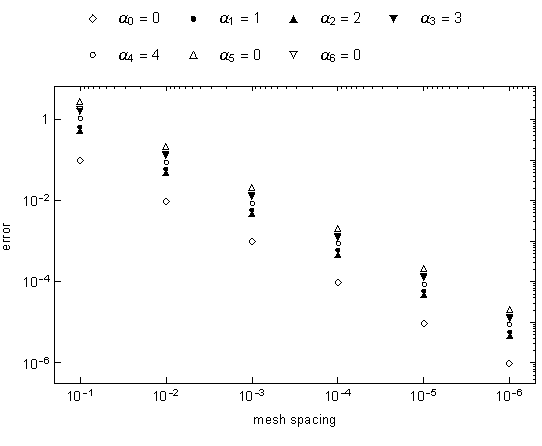
\includegraphics[ width = 3.0in ]{graphics/decay_rates_Cinf} 
   \caption{Error in computing the Legendre amplitudes for the function in \eqref{eqn:smooth function}.}
   \label{fig:legendre error}
\end{figure}


\textbf{Solution--}
Switch to the monomial basis $\paren{g_{k}(x) = x^{k}}$, and compute the amplitudes  using \eqref{eq:l:full}. Use an affine transformation to recover the Legendre amplitudes, for example $b=T_{6} a$. The algorithm is exact. The test case used $\Delta = 0.25$ for a double precision computation in \emph{Mathematica} and recovered exact answers\footnote{The exact answer is attributed to the twin blessings of a high quality linear solver and the $x$ values having exact binary representation.} for $\alpha_{0}-\alpha_{6}$.

\textbf{Source of error--}
The root of the error is analytic integrals do not equal their numeric counterparts; the off-diagonal elements in \eqref{eq:l:full} are not zero and the solution methods for \eqref{eq:l:lite} don't work. For example, the product function $P_{0}\paren{x} P_{2}\paren{x}$, which corresponds to $\A{*}\A{}$ matrix element $(r,c) = (1,3)$ in  \eqref{eq:L:full}, 
  % = =  e q u a t i o n
  \begin{equation}
    \int_{-1}^{1}{P_{0}\paren{x} P_{2}\paren{x} dx} \ne \sum_{\nu=0}^{2n} P_{0}\paren{x_{\nu}} P_{2}\paren{x_{\nu}} \Delta .
    %\label{eqn:}
  \end{equation}
  % = =
The left-hand side is an analytic integral exactly equal to 0 and the right-hand side is a numerical summation. For $\Delta = \frac{1} {4}$ the integral is approximated as
  % = =  e q u a t i o n
  \begin{equation*}
    \sum_{\nu=1}^{8} \frac{1}{2}  \paren{ 3x_{\nu}^{2} - 1 } \Delta = \frac{1}{64} \ne 0,
    %\label{eqn:}
  \end{equation*}
  % = =
a statement of orthogonality lost.
Figure \ref{fig:compare errors} contrasts the two integration methods.


\begin{figure}[htbp] %  figure placement: here, top, bottom, or page
   \centering
   \includegraphics[ width = 2.5in ]{graphics/"area cont"} \\[10pt]
   \includegraphics[ width = 2.5in ]{graphics/"area disc"} 
   \caption{Error in computing matrix cross terms. The function is $P_{0}(x)P_{2}(x)$.} % By construction, the analytic integral in $\bigL$ is 0.}
   \label{fig:compare errors}
\end{figure}


%  +++  +++  +++  +++  +++  +++  +++  +++  +++  +++  +++  +++  +++  +++  +++  +++  +++  +++  +++  +++  +++  +++  +++  +++
\subsubsection{\label{sec:infinity insurance}Example II: discontinuous function}
Stepping outside of the strictures of the Riesz--Fischer theorem, consider a discontinuous function,
  % = =  e q u a t i o n
  \begin{equation}
    \sgn x = 
    \begin{cases}
      \phantom{-}1 & x > 0 \\
      \phantom{-}0 & x = 0 \\
                -1 & x < 0
    \end{cases} .
    \label{eqn:sgn}
  \end{equation}
  % = =
The \href{http://mathworld.wolfram.com/Sign.html}{sign function} has odd parity so the approximation contains only odd terms.

Figure \ref{fig:signum approx} compares fits with maximum order $d=50$, $d=100$, and $d=200$ against the sign function. The amplitudes for the approximations are shown in Figures \ref{fig:signum approx amps monomial} and  \ref{fig:signum approx amps Legendre}. 

\begin{figure}[htbp] %  figure placement: here, top, bottom, or page
   \centering
   \includegraphics[ trim = 0.0cm 0cm 0cm 0.8cm, width = 2.5in ]{graphics/"approx col"}
   \caption{Approximation of the sign function showing the Gibbs phenomena at the midpoint and boundaries.}
   \label{fig:signum approx}
\end{figure}

Amplitudes for the monomial approximations are shown in Figure \ref{fig:signum approx amps monomial}. To use a logarithmic scale, the absolute value of the amplitude $\abs{a}$, is shown. Filled rectangles indicate the sign of the amplitude is positive, open rectangles indicate negative values. Amplitudes for even functions have value 0 and are not plotted. The amplitudes grow without bound. Notice the invariance in form of the amplitudes; the scale is changing, but not the shape.

Amplitudes for the Legendre approximations are shown in Figure \ref{fig:signum approx amps Legendre}. Positive values are shown with filled rectangles, 0 values with open diamonds, and negative values with open rectangles. These amplitudes are bounded. The plots demonstrate that the values of the lowest order terms do not change as the order of fit is increased. Notice the invariance of amplitude values; the lower order amplitudes do not change as the fit order increases.

%\break
%\clearpage

\begin{figure}[t] %  figure placement: here, top, bottom, or page
   \centering
   \includegraphics[ trim = 0.0cm 0cm 0cm 0.8cm, width = 3.05in ]{graphics/"M 0200"} 
   \caption{Amplitudes for the monomial approximation of the sign function in \eqref{eqn:sgn} found by solving \eqref{eq:l:full}.}
   \label{fig:signum approx amps monomial}
\end{figure}

\begin{figure}[t] %  figure placement: here, top, bottom, or page
   \centering
   \includegraphics[ trim = 0.0cm 0cm 0cm 0.8cm, width = 3.05in ]{graphics/"L 0200"} 
   \caption{Amplitudes for the Legendre approximation of the sign function in \eqref{eqn:sgn} found by solving \eqref{eq:l:full}.}
   \label{fig:signum approx amps Legendre}
\end{figure}

\textbf{Problem--}
Monomial amplitudes grow without bound quickly exhausting the range of double precision computation. In such cases, orthogonal polynomials provide infinity insurance; Legendre amplitudes are bound. The monomial linear system is ill-conditioned. After all, these functions are merely linearly independent. But the Legendre polynomials present a much better conditioned linear system as they are closer to being orthogonal in $\littlel$.

\textbf{Solution--}
Use the Legendre basis $\paren{g_{k}(x) = P_{k}(x)}$ and compute the amplitudes using \eqref{eq:l:full}. Affine transformations recover the monomial amplitudes, for example $a=T_{200}^{-1} b$.


%  +  +  +  +  +  +  +  +  +  +  +  +  +  +  +  +  +  +  +  +  +  +  +  +  +  +  +  +  +  +  +  +  +  +  +
\section{Conclusion}
Computation demands discrete evaluation and finite meshes. Outside of sine and cosine, there are no functions continuous in both $\bigL$ and $\littlel$. The presumption of orthogonality in discrete space introduces extreme numerical errors. Instead, rely upon linear independence to create and solve the linear systems. Affine transformations connect the function spaces of choice. When resolving discontinuous functions, $\bigL-$orthogonal functions can create a dense linear system with improved conditioning.

One of the authors (PFE) thanks Los Alamos for support during the summer of 2012.

%  +  +  +  +  +  +  +  +  +  +  +  +  +  +  +  +  +  +  +  +  +  +  +  +  +  +  +  +  +  +  +  +  +  +  +
\input{sections/"bibliography csc 15"}

\end{document}